\documentclass[11pt]{article}

\title{$1}
\author{Nikolas Eptaminitakis}

\usepackage[T1]{fontenc}
\usepackage{librefranklin}
\renewcommand*\familydefault{\sfdefault} %% Only if the base font of the document is to be sans serif



% Margins
 \setlength{\oddsidemargin}{0 in}
 \setlength{\evensidemargin}{0 in}
 \setlength{\textwidth}{6.6 in}
 \setlength{\topmargin}{0 in}
 \setlength{\textheight}{8.55 in}
\setlength{\headheight}{0.18 in}

% Packages  
%\usepackage[margin=0.8 in]{geometry} % decides size of margins, paper etc
%\usepackage{palatino} % a font
\usepackage{hhline}
%\usepackage{forest}
\usepackage{cancel} % to cross out stuff
\usepackage{amsmath}
\usepackage{marginnote}  % to put notes on the margins
\usepackage{amssymb}
\usepackage{amsthm}
\usepackage{accents}
\usepackage{amsfonts}
\usepackage{mathtools}
\usepackage{enumerate}
%\usepackage{verbatim}
\usepackage{comment}
%\usepackage{makeidx}
\usepackage{hyperref}
\usepackage{multirow}
\usepackage[noadjust]{cite}
\usepackage{color}
\usepackage{pst-node}
\usepackage{tikz-cd} 
\usepackage[toc,page]{appendix}			% table of contents


% Global options
\allowdisplaybreaks
\mathtoolsset{showonlyrefs}


% Math Operators
\DeclareMathOperator{\sgn}{sgn}
\DeclareMathOperator{\pv}{pv}
\DeclareMathOperator{\Div}{div}
\DeclareMathOperator{\Int}{int}
\DeclareMathOperator{\dist}{dist}
\DeclareMathOperator{\sech}{sech}
\DeclareMathOperator{\sing}{sing}
\DeclareMathOperator{\supp}{supp}
\DeclareMathOperator{\sign}{sign}
\DeclareMathOperator{\II}{II}
\DeclareMathOperator{\diag}{diag}
\DeclareMathOperator{\trace}{tr}
\DeclareMathOperator{\grad}{grad}
\DeclareMathOperator{\adj}{adj}
\DeclareMathOperator{\Span}{span}
\DeclareMathOperator{\Sym}{Sym}
\DeclareMathOperator{\arcsinh}{arsinh}
\DeclareMathOperator{\artanh}{artanh}
\DeclareMathOperator{\proj}{proj}
\DeclareMathOperator{\arcosh}{arcosh}
\DeclareMathOperator{\Diff}{Diff}

%Special Characters
\let \sectionsymbol \S
\renewcommand{\P}{\mathbb{P}}
\newcommand{\R}{\mathbb{R}}
\newcommand{\B}{\mathbb{B}}
\newcommand{\C}{\mathbb{C}}
\renewcommand{\S}{\mathbb{S}}
\renewcommand{\H}{\mathbb{H}}
\newcommand{\Z}{\mathbb{Z}}
\newcommand{\pr}{\mathcal{p}\mathcal{r}}
\newcommand{\ru}{{\sqrt{u}}}
\newcommand{\SM}{\overline{S^*M}}
\newcommand{\pdo}{\Psi\text{DO}}
\newcommand{\ox}{\o{\xi}}
\newcommand{\tM}{\tilde{M}}
\newcommand{\tg}{\tilde{g}}
\newcommand{\p}{\partial}
\newcommand{\n}{\nabla}
\newcommand{\on}{\overline{\n}}
\newcommand{\tn}{\tilde{\nabla}}
\newcommand{\oM}{\overline{M}}
\newcommand{\tX}{\widetilde{X}}
\newcommand{\ta}{{\widetilde{\alpha}}}
\newcommand{\tx}{{\widetilde{x}}}
\newcommand{\oX}{\overline{X}}
\newcommand{\X}{\mathfrak{X}}
\newcommand{\oW}{\overline{W}}
\newcommand{\oT}{\overline{T}}
\newcommand{\tf}{\tilde{f}}
\newcommand{\tr}{\tilde{\r}}
\newcommand{\x}{{x_c}}
\newcommand{\oU}{\overline{U}}
\newcommand{\oH}{\overline{H}}
\newcommand{\oSU}{\o{S^*U}}
\newcommand{\oSH}{\overline{S^*\mathbb{H}^2}}
\newcommand{\rg}{\rangle}
\renewcommand{\lg}{\langle}
\newcommand{\bTM}{{}^bT^*\oM}
\newcommand{\Di}{\Delta\iota}
\newcommand{\hx}{\hat{\xi}}
\newcommand{\ba}{\breve{a}}
\newcommand{\tz}{\widetilde{\zeta}}
\newcommand{\hY}{\hat{Y}}
\newcommand{\tPhi}{\widetilde{\Phi}}
\newcommand{\og}{\overline{\g}}
\newcommand{\prl}{\parallel}
\newcommand{\cM}{\mathring{M}}
\newcommand{\bA}{\mathbf{A}}
\newcommand{\bx}{\mathbf{x}}
\newcommand{\bv}{\mathbf{v}}
\newcommand{\bI}{\mathbf{I}}


% Calligraphic letters

\newcommand{\calA}{\mathcal{A}}
\newcommand{\calB}{\mathcal{B}}
\newcommand{\calC}{\mathcal{C}}
\newcommand{\calD}{\mathcal{D}}
\newcommand{\calE}{\mathcal{E}}
\newcommand{\calF}{\mathcal{F}}
\newcommand{\calG}{\mathcal{G}}
\newcommand{\calH}{\mathcal{H}}
\newcommand{\calL}{\mathcal{L}}
\newcommand{\calO}{\mathcal{O}}
\newcommand{\calR}{\mathcal{R}}
\newcommand{\calS}{\mathcal{S}}
\newcommand{\calU}{\mathcal{U}}
\newcommand{\calV}{\mathcal{V}}
\newcommand{\calW}{\mathcal{W}}
\newcommand{\calY}{\mathcal{Y}}
\newcommand{\calZ}{\mathcal{Z}}


%Greek Letters

\renewcommand{\a}{\alpha}
\renewcommand{\b}{\beta}
\newcommand{\g}{\gamma}
\renewcommand{\d}{\delta}
\let\epsilon\varepsilon
\newcommand{\e}{\epsilon}
\newcommand{\h}{\eta}
\newcommand{\z}{\zeta}
\newcommand{\smsec}{\G_0^{\frac{1}{2}}}
\newcommand{\G}{\Gamma}
\newcommand{\oG}{\overline{\Gamma}}
\renewcommand{\r}{\rho}
\renewcommand{\t}{\tau}
\renewcommand{\k}{\kappa}
\renewcommand{\l}{\lambda}
\newcommand{\s}{\sigma}
\renewcommand{\th}{\theta}
\newcommand{\om}{\omega}
\newcommand{\w}{\omega}
\renewcommand{\oe}{\overline{\eta}}
\newcommand{\tU}{\tilde{U}}

% Environments

\newtheorem{definition}{Definition}
\newtheorem{lemma}{{Lemma}}
\newtheorem{theorem}{Theorem}
\newtheorem{proposition}{Proposition}
\newtheorem{conjecture}{Conjecture}
\newtheorem{remark}{Remark}
\newtheorem{corollary}{Corollary}
\newtheorem{example}{Example}
\newtheorem{ansatz}{Ansatz}
\newtheorem{problem}{Problem}
\newtheorem{question}{Question}
\newenvironment{solution}{\paragraph{Solution:}}{\hfill$\square$}
\newtheorem{goal}{Goal}
\newtheorem{claim}{Claim}
\newtheorem{idea_that_doesnt_work}{Idea that doesn't work}
\newtheorem{unverified_claim}{Unverified Claim}
\newenvironment{answer}{\paragraph{Answer:}}{\hfill$\square$}


\let \o \undefined
\def \o#1{\overline{#1}}
\def\fr#1#2{\frac{#1}{#2}}
\def\tt#1{\textit{#1}}

% \let\printintex\undefined
% \let\see\undefined

\let\td\undefined
\def \td#1{\widetilde{#1}}
\let\implies\Rightarrow

\begin{document}
\section*{Midterm 1 Practice Problems}

\noindent\textbf{Reminder:} For the midterm you are allowed to use a double-sided, \textbf{handwritten}, $8.5\times11'$ (letter sized)  note  sheet. If it is needed for the exam, the table of Laplace transforms as it appears in the textbook will be given.

Textbook Sections Covered: 
\begin{itemize}
    \item From Chapter 5: 5.1, 5.2, 5.3, 5.5
    \item From Chapter 6: 6.1, 6.2, 6.3, 6.4
    \item From Chapter 7: 7.1, 7.2 
\end{itemize}



\noindent Below, symbols in \textbf{boldface} indicate vectors or matrices. Primes indicate derivative with respect to $t$. The problems below offer an overview of the most important types of problems appearing in the sections above; \textit{you are not expected to be able to complete all of the problems below in one hour}.

\begin{enumerate}
    % \item Maybe show that set of vectors are linearly independent
    \item You are given the system 
    \begin{equation}\label{eq1}
        \begin{cases}
            x_1'=x_1-5x_2\\
            x_2'=x_1+3x_2
        \end{cases}.
    \end{equation}
    \begin{enumerate}
        \item  Find a pair of linearly independent solutions for \eqref{eq1}.
        Each of the two solutions you find should be a pair of the form $(x_1(t),x_2(t))$ with $x_1(t)$ and $x_2(t)$ \textbf{real valued functions.} 
        Make sure to check linear independendence as part of your solution.
        \item Which of the phase plane portraits below corresponds to \eqref{eq1}?
        \begin{figure}[h]
            \minipage{0.32\textwidth}
              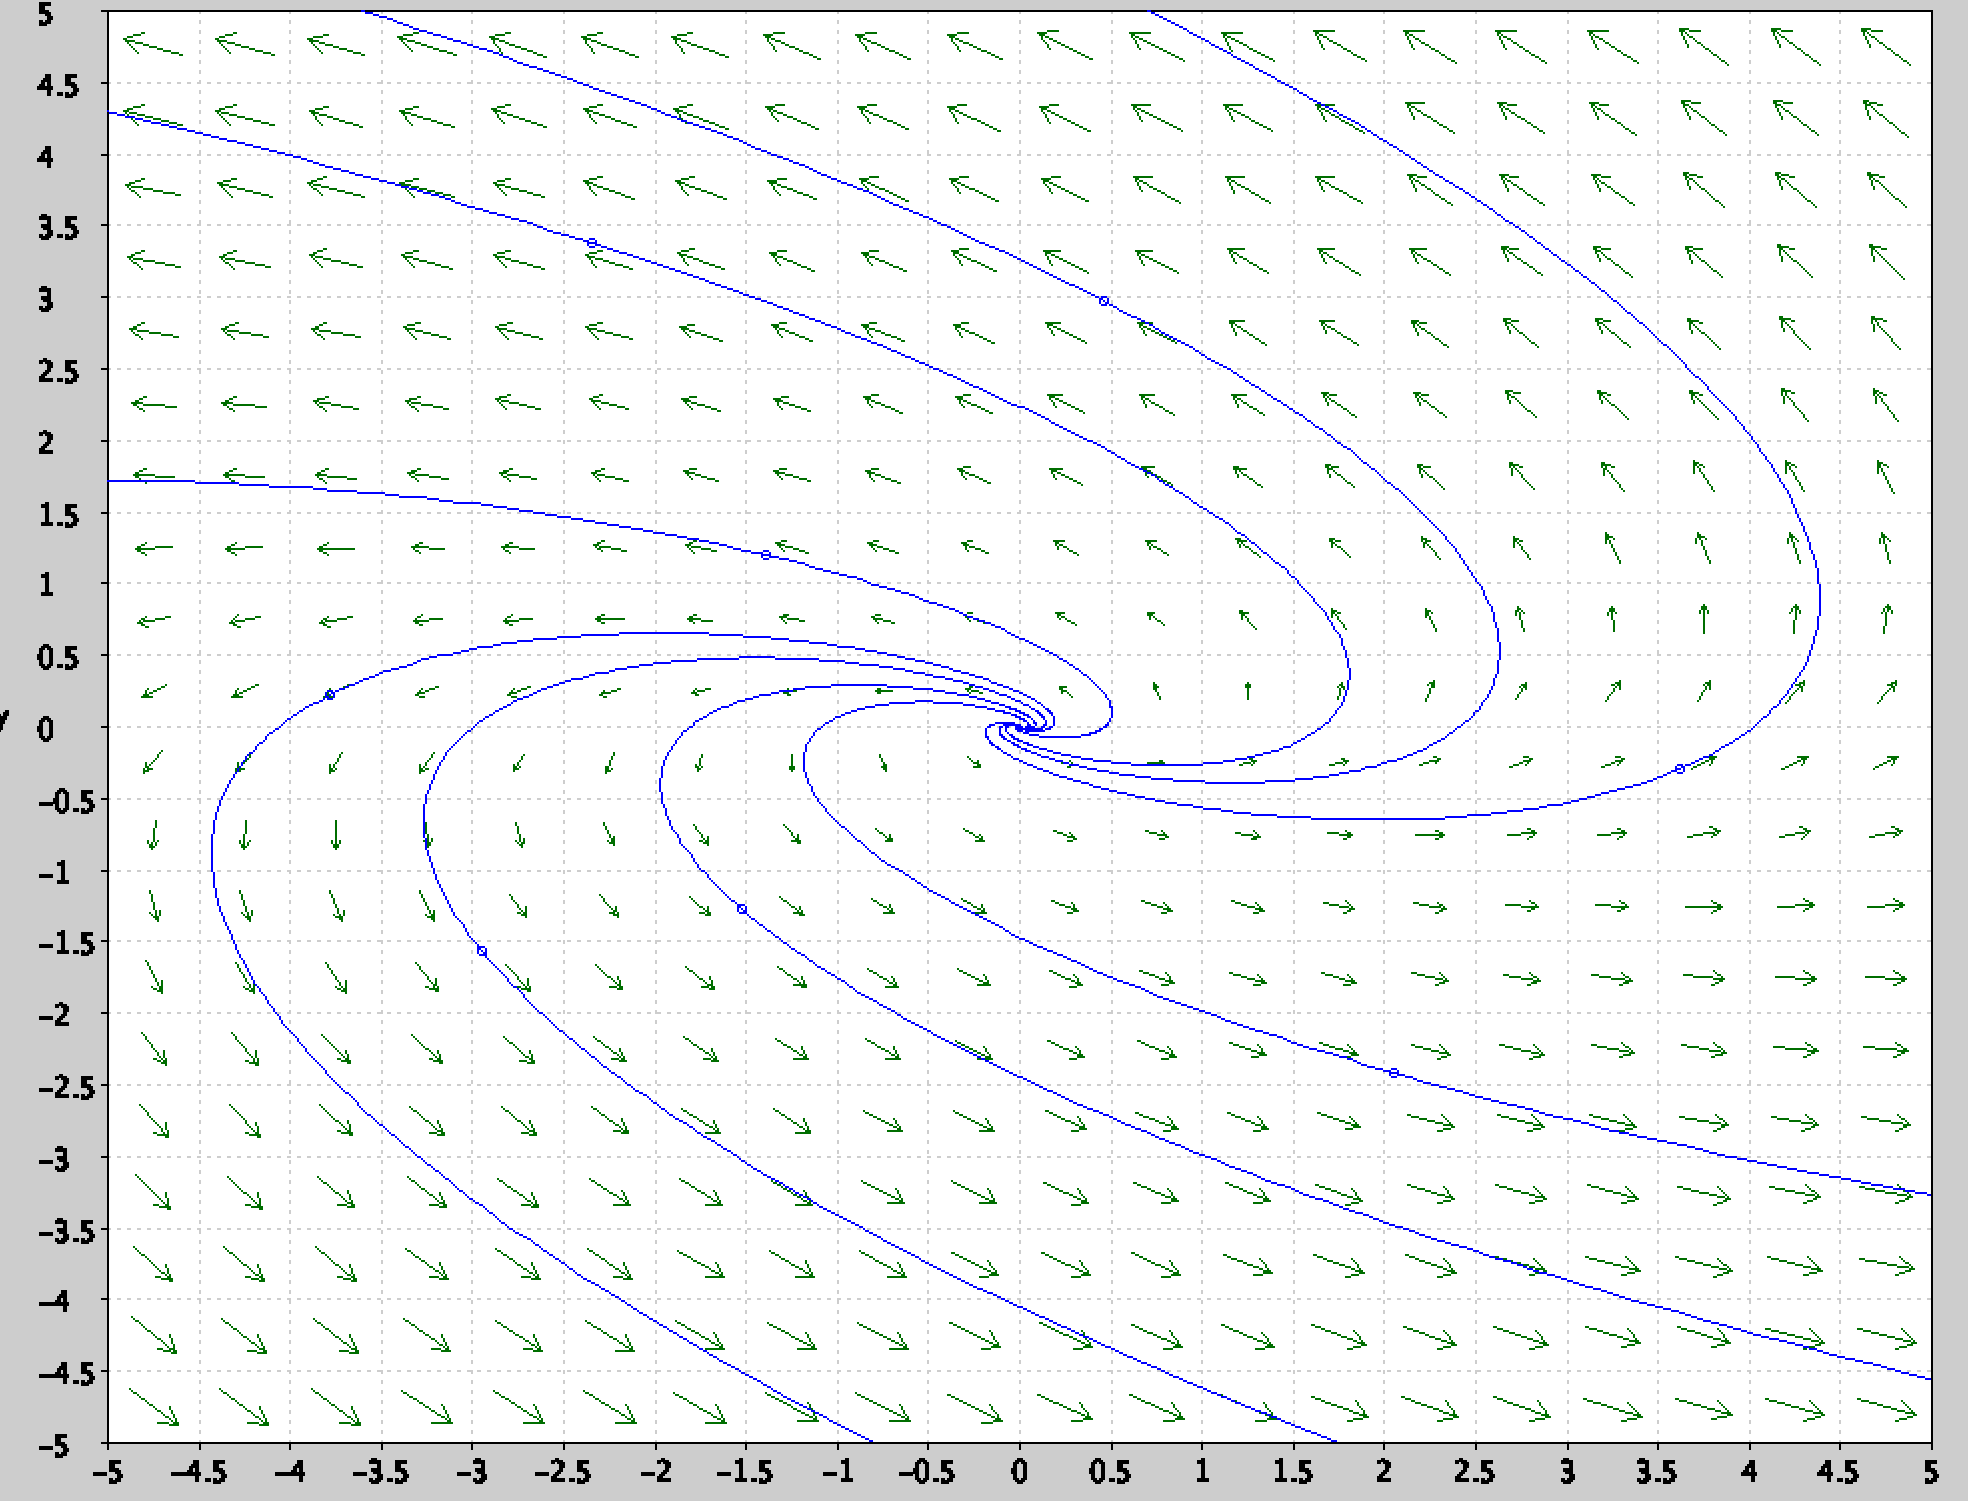
\includegraphics[width=\linewidth]{fig1}
              \caption{A.}
              % \label{}
        \endminipage\hfill
            \minipage{0.32\textwidth}
              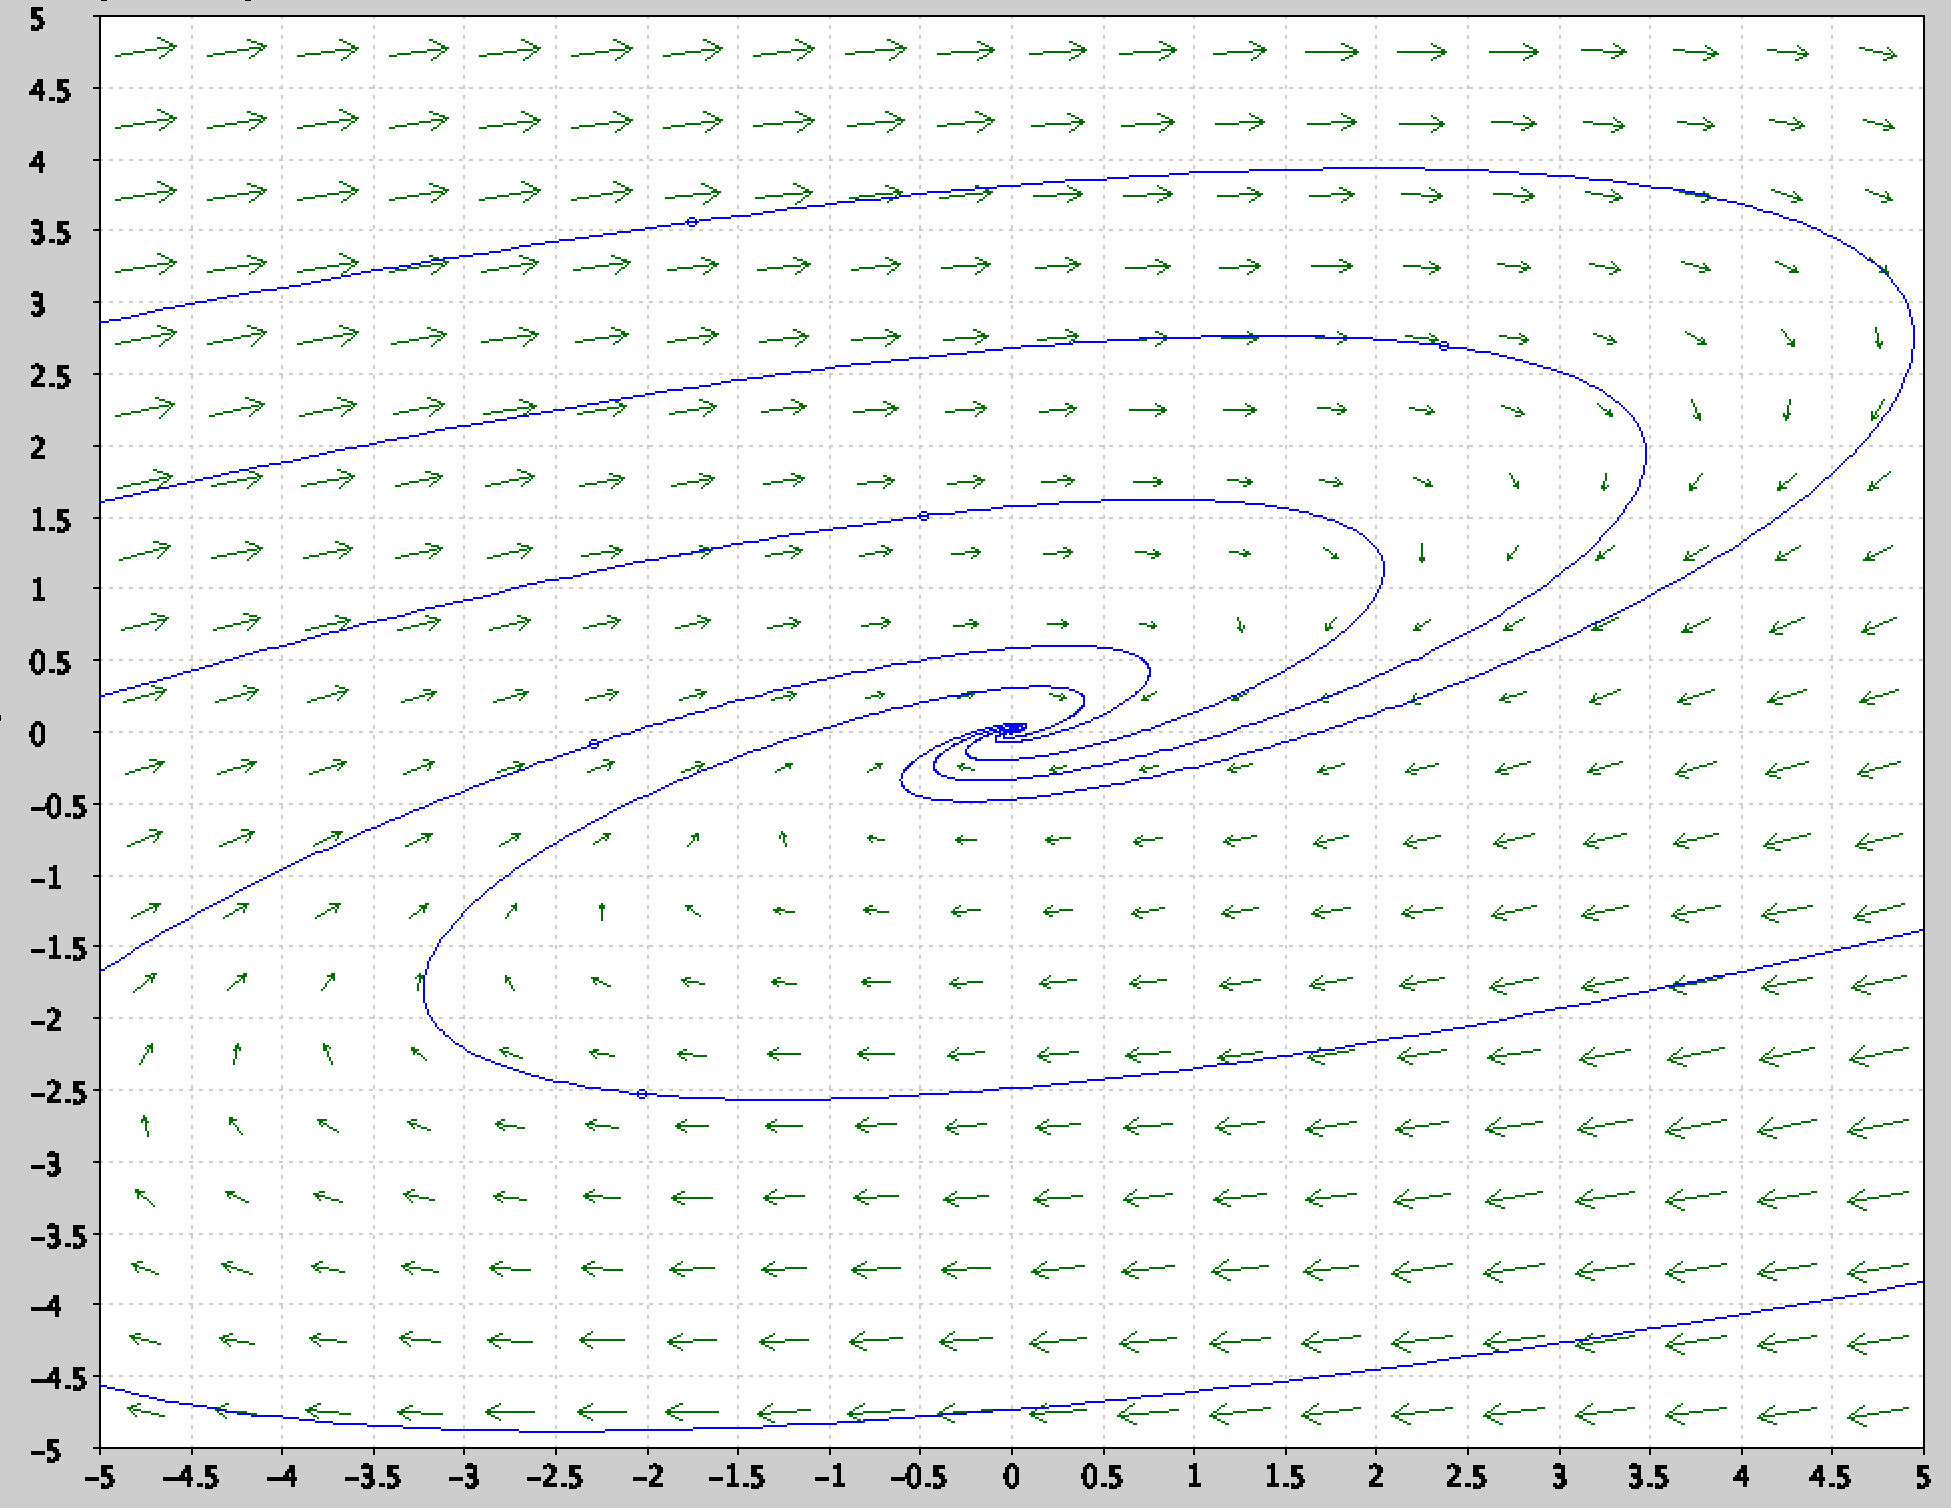
\includegraphics[width=\linewidth]{fig2}
              \caption{B.}
              % \label{}
        \endminipage\hfill
            \minipage{0.32\textwidth}
              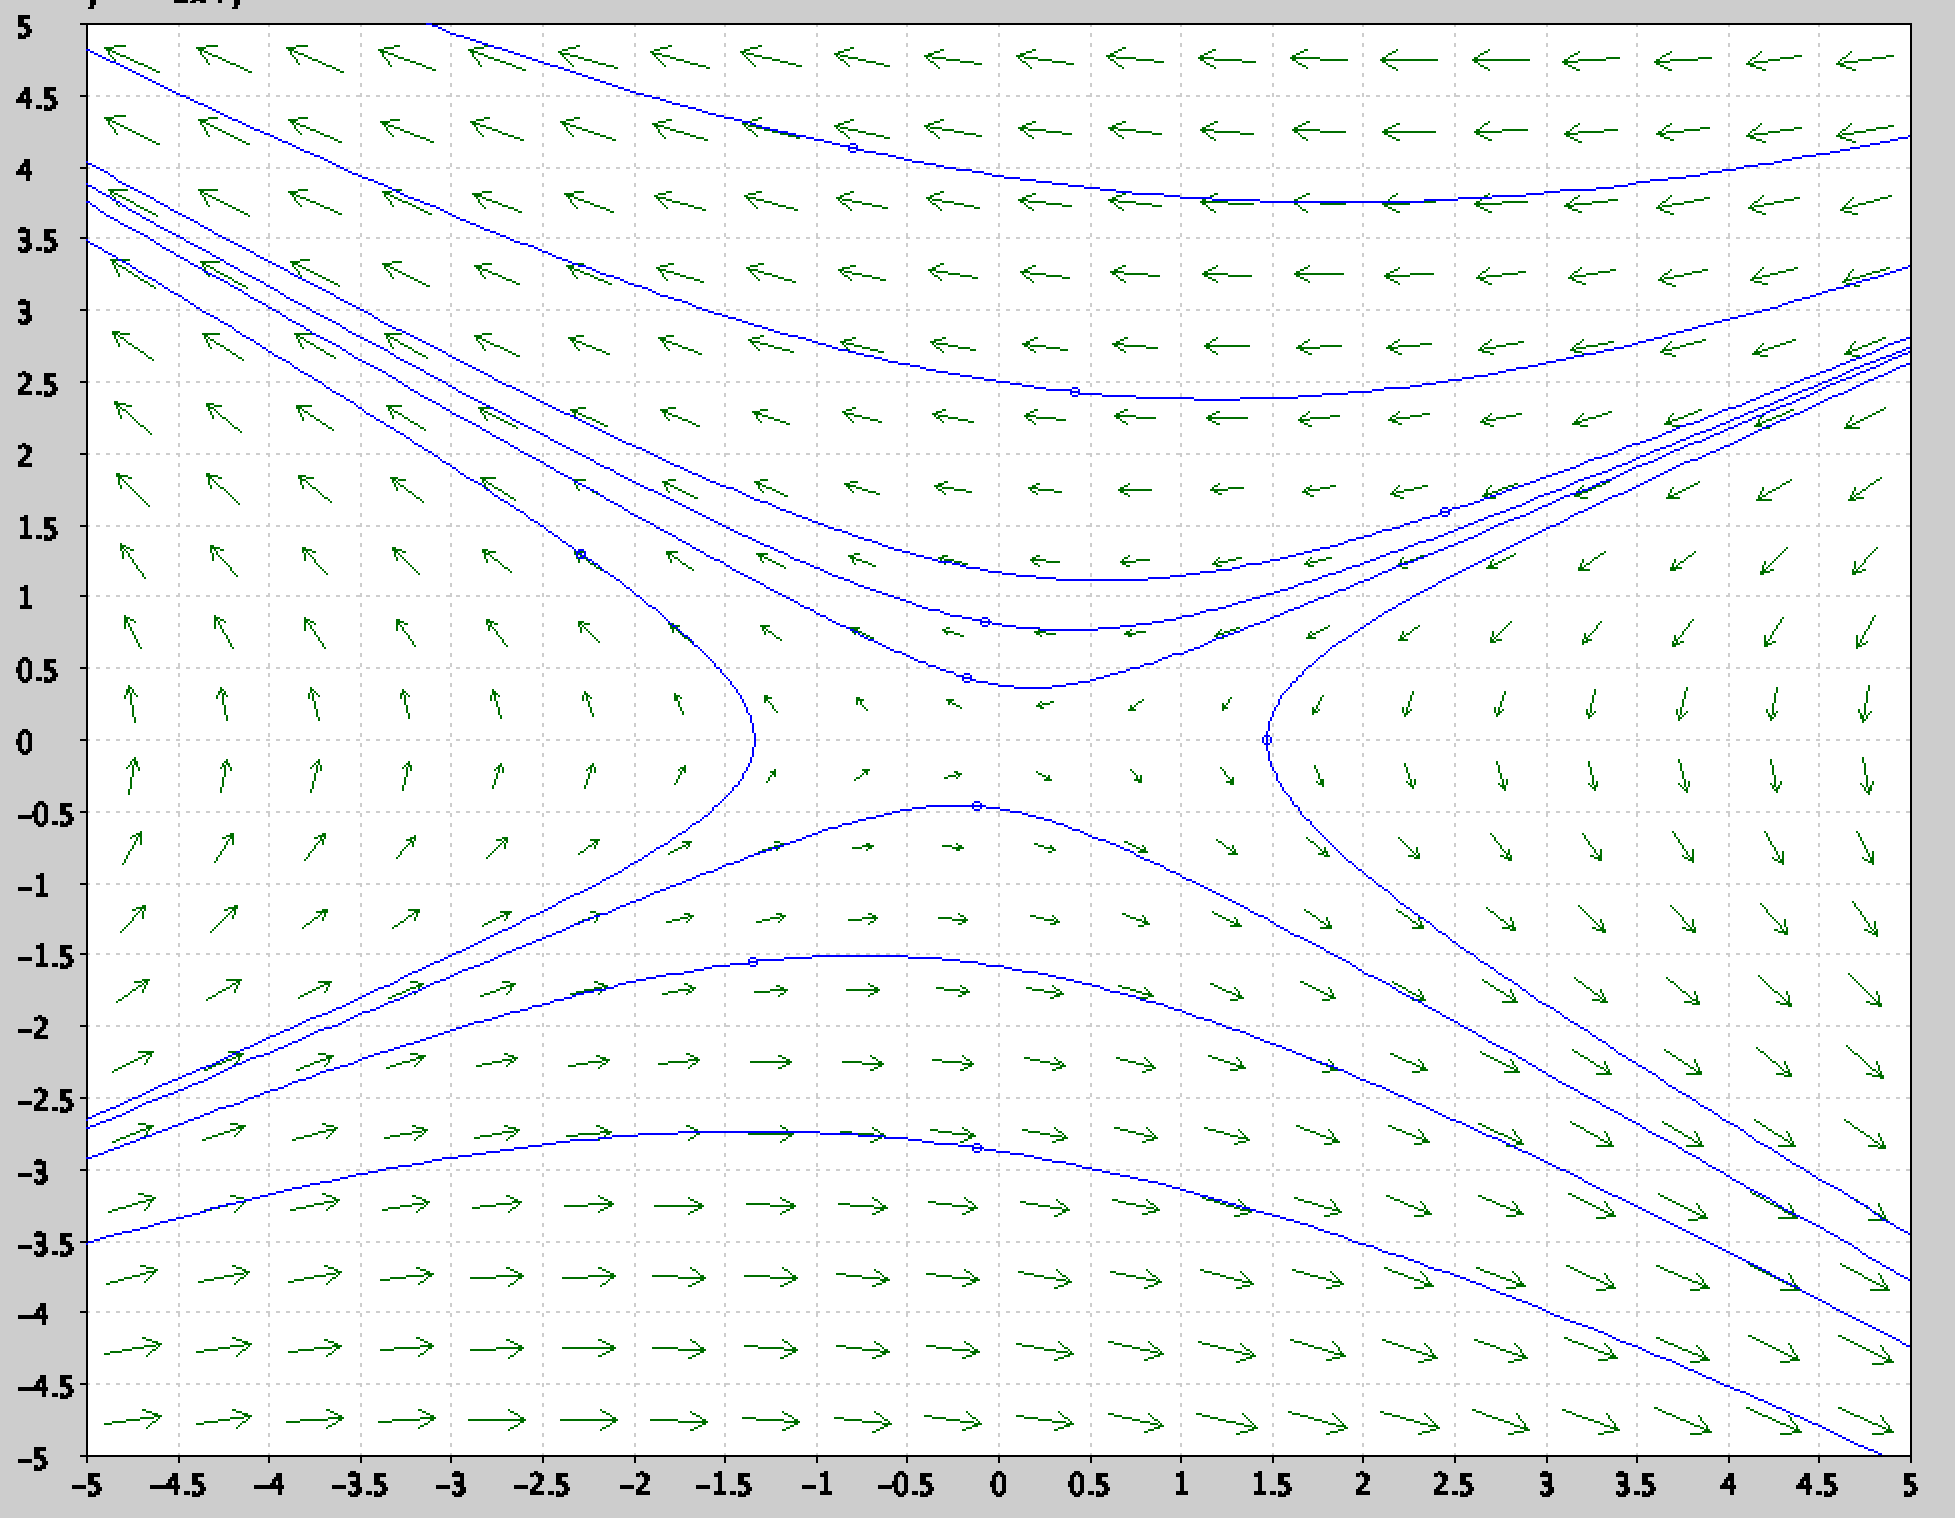
\includegraphics[width=\linewidth]{fig3}
              \caption{C.}
              % \label{}
            \endminipage
                    \end{figure}
    \end{enumerate}

    %  5.2 problem 12

    \item Find the solution of the system 
    \begin{equation}
        \begin{cases}
        x_1'=4x_1+x_2\\
        x_2'=6x_1-x_2
        \end{cases}
        % 
    \end{equation}
    which satisfies $x_1(0)=2$ and $x_2(0)=-1$.

    % 5.2 Problem 4
    
    \item You are given the system $\bx'=\bA\bx$, where 
    $$\bA=
        \left[
\begin{array}{ccc}
 -15 & -7 & 4 \\
 34 & 16 & -11 \\
 17 & 7 & 5 \\
\end{array}
\right].
    $$
Compute the general solution of the system. The following information is given:
\begin{itemize}
    \item $\bA$ has the eigenvalue $\l=2$ with multiplicity 3.
    \item The following matrix powers are given:
    \begin{equation}
        \hspace{-.5 in}\left[
\begin{array}{ccc}
 -17 & -7 & 4 \\
 34 & 14 & -11 \\
 17 & 7 & 3 \\
\end{array}
\right]^2=\left[
\begin{array}{ccc}
 119 & 49 & 21 \\
 -289 & -119 & -51 \\
 0 & 0 & 0 \\
\end{array}
\right]    ,\qquad\left[
\begin{array}{ccc}
 -17 & -7 & 4 \\
 34 & 14 & -11 \\
 17 & 7 & 3 \\
\end{array}
\right]^3= \left[
\begin{array}{ccc}
 0 & 0 & 0 \\
 0 & 0 & 0 \\
 0 & 0 & 0 \\
\end{array}
\right].
    \end{equation}
\end{itemize}

%  5.5 Problem 28




\item You are given the nonlinear system
\begin{equation}
\begin{cases}\label{nonlinear}
    \frac {dx}{dt}=F(x,y)=ye^{x+y}\\
    \frac {dy}{dt}=G(x,y)=-xe^{x+y}
\end{cases}
\end{equation}
\begin{enumerate}    
    \item Show that $(0,0)$ is a critical point for the system \eqref{nonlinear}.
    \item \label{p2} Compute the linearization of \eqref{nonlinear} at the origin. What does the phase plane portrait of the \textit{linearized} system look like?
    \item What does Part \ref{p2} imply about the phase plane portait of the \textit{nonlinear} system \eqref{nonlinear} near the origin?
    \item Solve the equation 
    \begin{equation}
        \frac{dy}{dx}=\frac{G(x,y)}{F(x,y)}
    \end{equation}
    to find the trajectories of \eqref{nonlinear} in implicit form. Based on your answer, determine what the phase plane portrait of \eqref{nonlinear} looks like near the origin.
\end{enumerate}

\item You are given the \textit{linear} system 
\begin{equation}
    \begin{cases}\label{parameter}
    \frac {dx}{dt}=4x+\e y\\
    \frac {dy}{dt}=x-y
\end{cases}
\end{equation}
depending on a linear parameter $\e$.
Determine the values of $\e$ for which the phase plane portrait of \eqref{parameter} is an unstable node.


\item 

You are given the following system
\begin{equation}
    \begin{cases}\label{parameter}
    \frac {dx}{dt}= 7x-x^2+xy\\
    \frac {dy}{dt}=y-4xy
\end{cases}
\end{equation}
describing two animal populations.
\begin{enumerate}
    \item Is the relationship between them one of cooparation, predation or competition? In case of predation determine which population is the prey and which one is the predator.
    \item Find the physically relevant critical points of the system.
    \item Suppose we start with initial conditions $x=2$ and $y=4$. Based on the phase plane portrait below, what is the long term behavior of the system?
    \begin{figure}[h]
    \begin{center}
        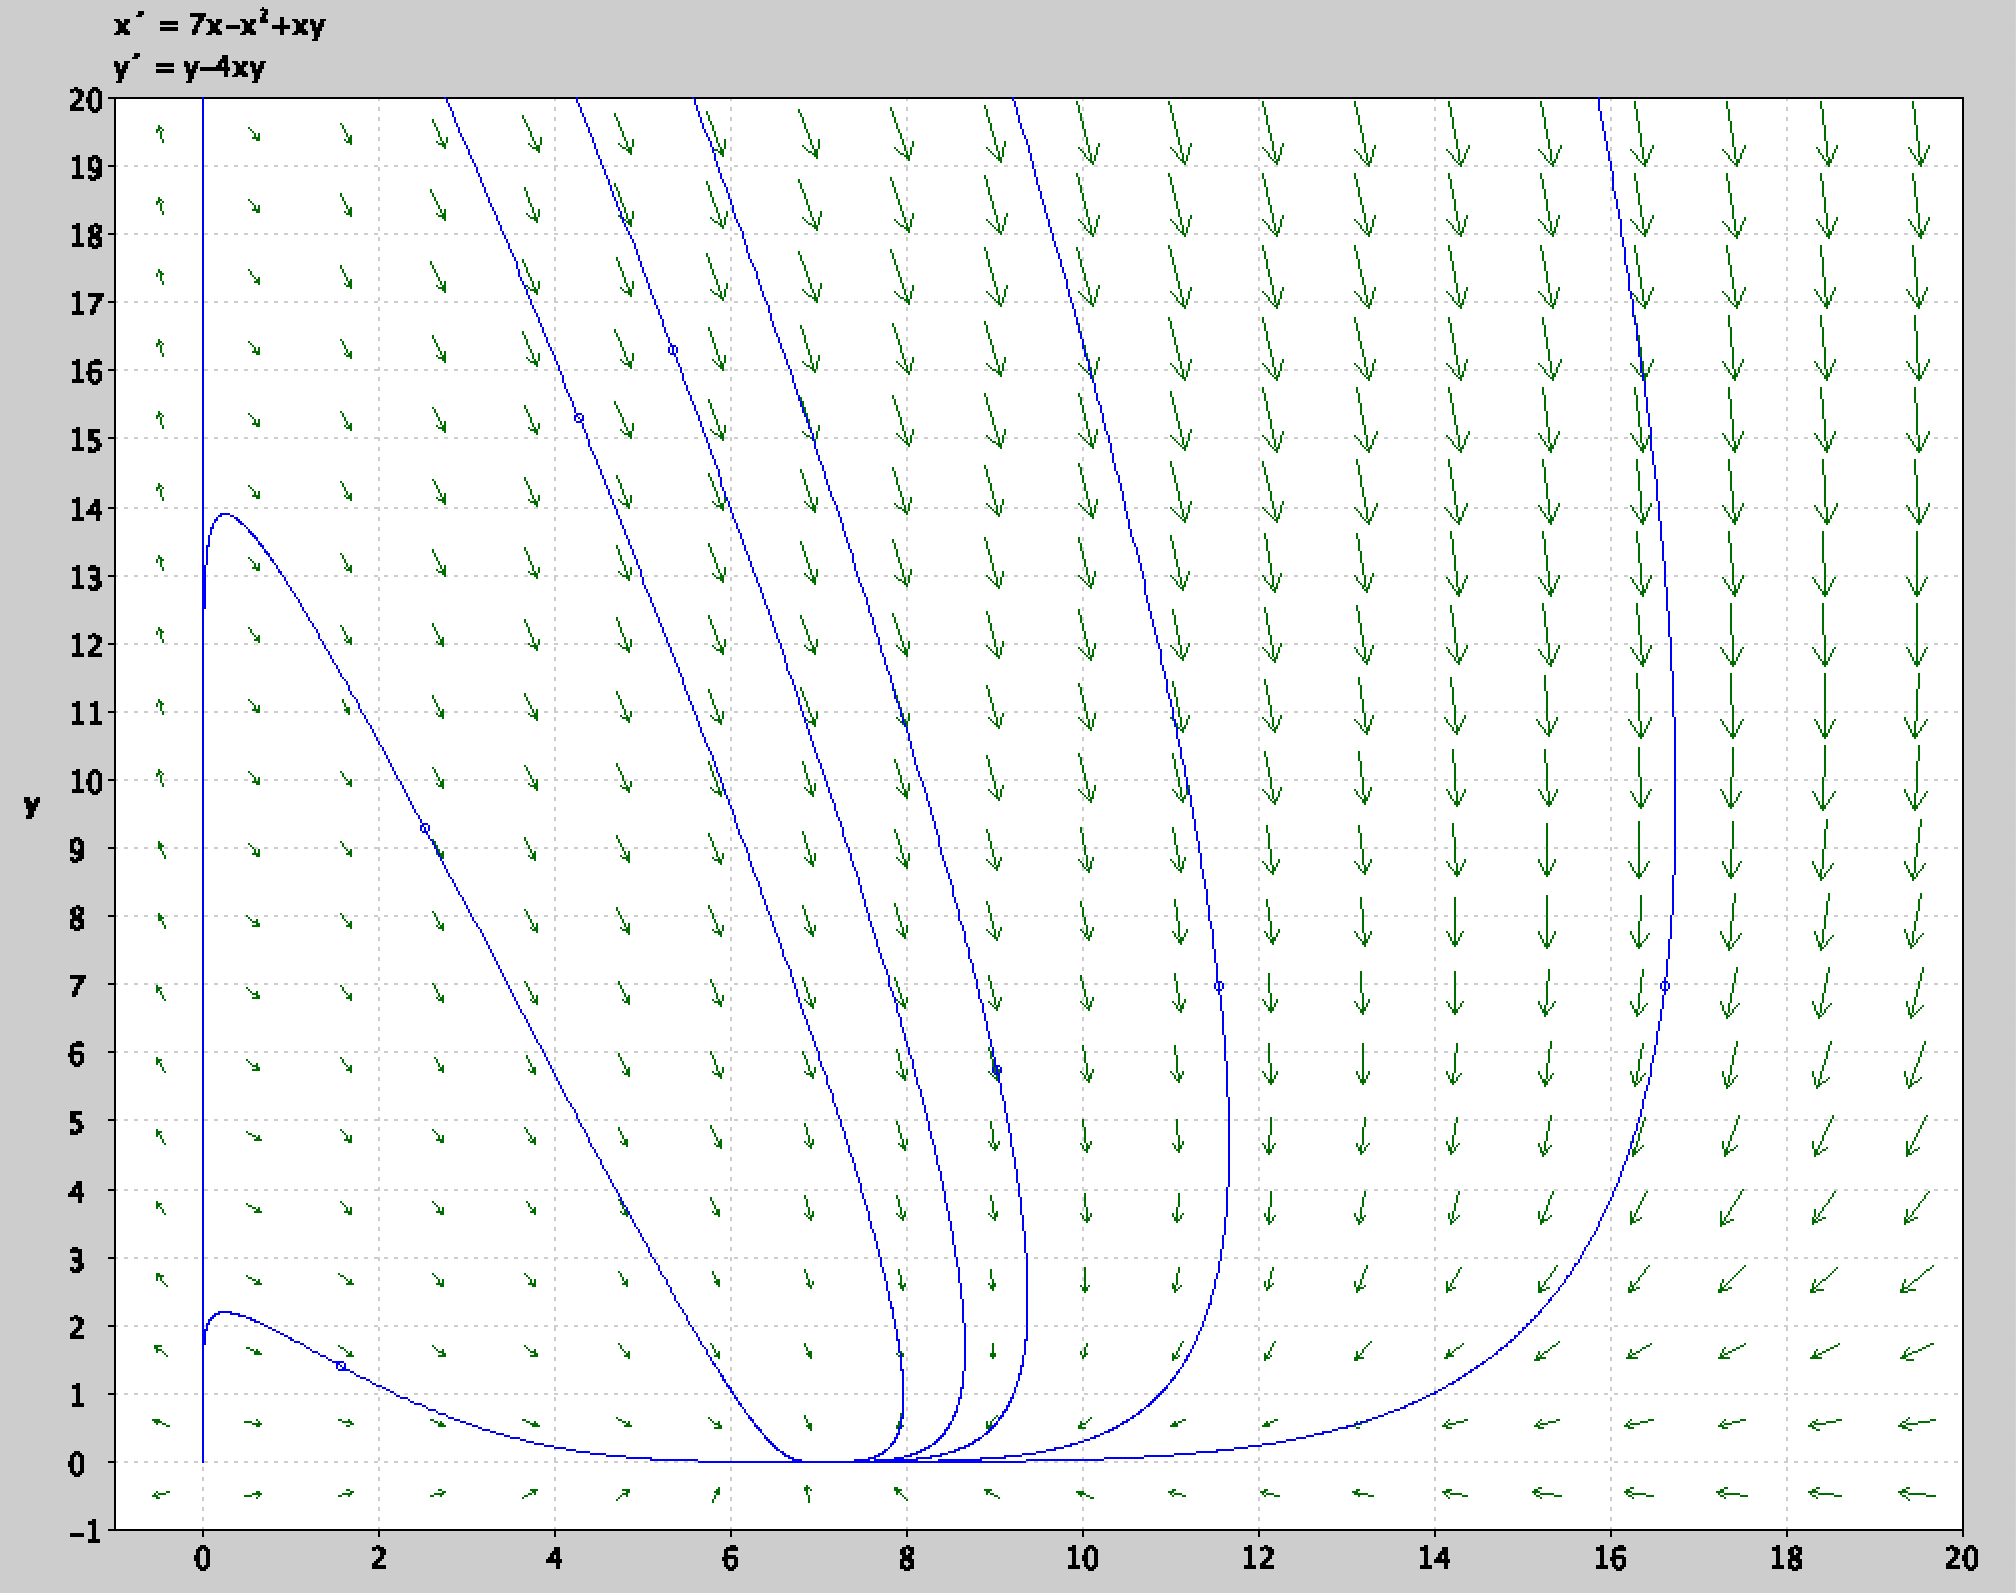
\includegraphics[scale=.2]{Phase_plane_portrait.png}
        \end{center}
    \end{figure}
        
\end{enumerate}


\item The equation $x''+4x-5x^3+x^5=0$  corresponds to a mass and spring system in which we retain the 3rd and 5th degree terms of the spring force function.
Turn this equation into an equivalent 1st order system and determine all equilibrium solutions.

\item Compute the Laplace transform $F(s)=\calL\{f(t)\}$, where $f(t)=\sinh(t)$ from the definition, i.e. without using a table (recall that $\sinh(t)=\frac{1}{2}(e^t-e^{-t})$).
For what $s$ is $F(s)$ defined?


\item Use the Laplace Transform to solve initial value problem
\begin{equation}
    \begin{cases}
        x'=2x+y\\
        y'=6x+3y
    \end{cases}
\end{equation}
under the initial conditions $x(0)=1$, $y(0)=-2$.

% 7.2 problem 11























\item * It was mentioned in lecture that when you are trying to find a chain of generalized eigenvectors of length $k$ based on a true eigenvector for a matrix $A$ with eigenvalue $\l$ of high defect you should start from the top instead of the bottom.
That is, you should first find a generalized eigenvector $\bv_k$ of the rank $k$ and go down the ``ladder''
\begin{equation}
        \label{eq:chain}
    % 
    \begin{aligned}
        % 
        &(\bA-\l \bI)\bv_{k}=\bv_{k-1}\\
        &\dots\\
        &(\bA-\l \bI)\bv_{3}=\bv_{2}\\
        &(\bA-\l \bI)\bv_{2}=\bv_{1}
    \end{aligned}
\end{equation} until you reach a true eigenvector, instead of starting with a true eigenvector and trying to find a chain based on it by working your way up.
The reason the ``bottom-to-top'' approach does not always work has to do with the fact that the matrix $\bA-\l\bI$ is singular, and the last equation in \eqref{eq:chain} might not be solvable for $\bv_2$.
The following exercise demonstrates what can go wrong.

Suppose that we have the matrix
\begin{equation}
    \bA=\left[
\begin{array}{cccc}
 3 & 1 & 0 & 0 \\
 0 & 3 & 1 & 0 \\
 0 & 0 & 3 & 0 \\
 0 & 0 & 0 & 3 \\
\end{array}
\right]
\end{equation}
\begin{enumerate}
    \item Check that $\l=3$ is an eigenvalue of multiplicity 4 and defect 2.
    \item Check that $\bv_1=[0,0,0,1]^T$ is an eigenvector.
    \item What happens if you try to find a chain of generalized eigenvectors based on $\bv_1$ by starting from $\bv_1$ and trying to work your way up using \eqref{eq:chain}?

    \item Find the general solution of the system $\bx'=\bA\bx$.
    You are given the following:
    \begin{equation}
        \left[
\begin{array}{cccc}
 0 & 1 & 0 & 0 \\
 0 & 0 & 1 & 0 \\
 0 & 0 & 0 & 0 \\
 0 & 0 & 0 & 0 \\
\end{array}
\right]^2=\left[
\begin{array}{cccc}
 0 & 0 & 1 & 0 \\
 0 & 0 & 0 & 0 \\
 0 & 0 & 0 & 0 \\
 0 & 0 & 0 & 0 \\
\end{array}
\right],\quad  \left[
\begin{array}{cccc}
 0 & 1 & 0 & 0 \\
 0 & 0 & 1 & 0 \\
 0 & 0 & 0 & 0 \\
 0 & 0 & 0 & 0 \\
\end{array}
\right]^3=\left[
\begin{array}{cccc}
 0 & 0 & 0 & 0 \\
 0 & 0 & 0 & 0 \\
 0 & 0 & 0 & 0 \\
 0 & 0 & 0 & 0 \\
\end{array}
\right].
    \end{equation}
\end{enumerate}

%  Handout example 1

\end{enumerate}


\end{document}